%%% 左右余白が3cmもある. p1の上部の空白が数行分多い
\documentclass{interim} % 中間用 clsファイル
\usepackage[dvipdfmx]{graphicx}
\usepackage{amsmath}
\usepackage{comment}
\usepackage{amsfonts}
\chukantitle % タイトル

% タイトル
\date{2022年 9月 29日}
\thisevent{2022年度 \ I類(情報系) \ コンピュータサイエンスプログラム \ 卒業研究中間発表会}
\title{動的に要素が変化する多重集合に対するMin-hashの空間計算量の削減}
\mymajor{先端工学基礎課程}
\mylab{古賀研究室}
\mynum{1920031}
\myname{山川 竜太郎}

\renewcommand{\baselinestretch}{0.928}

\begin{document}
\maketitle

\section{はじめに}
近年、IoTやSNSの発展に伴いストリームデータが取り扱われる機会が増え、ストリームデータを対象とする類似検索の重要性が増している。類似検索ではストリームデータを要素が動的に変わる集合とみなし、集合間類似検索により、類似ストリームデータを探す。集合間類似度としてはJaccard係数が良く用いられる。しかし、集合が変わるたびにJaccard係数を計算しなおすのはオーバーヘッドが大きい。そのため、各集合に対するコンパクトなスケッチをMin-Hashというハッシュ関数により生成し、スケッチ間でJaccard係数を近似計算する手法が提案されている。本研究では、「データストリームを対象とした動的多重集合に対するMin-hashの高速計算アルゴリズム」の研究を引継いでいる。\cite{RP}

\subsection{Min-hash}
集合に対する確率的なハッシュ関数である。Jaccard係数の算出を高速化するために、Min-hashは計算されたハッシュ値が一致する確率はJaccard係数と一致するという性質を持ち、それを利用する。(\ref{RP1})

\begin{eqnarray}
	\label{RP1}
	Pr[h(A)=h(B)]=\frac{A\cap	B}{A\cup B}
\end{eqnarray}

集合に対する類似検索をハッシュテーブルで実現可能である。

式(\ref{RP1})でhはハッシュ関数であり、A,Bは集合である。
Min-hashによるハッシュ値の計算方法は、$Φ=\{x_1,x_2,…x_{|Φ|}\}$をアルファベット集合としたとき、ハッシュ関数はΦの各アルファベットに対して$\{1,2,…|Φ|\}$ の中から被らないようにランダムな値を割り当てることで決定される。1つのある集合の中のアルファベットを見て、その中の要素に対応する割り当て値の中から最小値を選ぶ。最小値がMin-hashによるハッシュ値となる。

\subsection{スライディングウインドウモデル}
スライディングウインドウモデルは、データストリームの直近W個の要素をスライディングウインドウと定義し、時刻が進むとウインドウに到着データを追加し、ウインドウ内の最古のデータを破棄する手法である。

\subsection{多重集合}
一般にオブジェクトの集まりを集合と呼ぶ.例えば{a, b, c}はアルファベットを要素とする集合である。一般的には要素群を表すアルファベットϕに対して、その要素を0 個以上含むものが集合となる。通常、集合は同じ種類の要素を1つしか含まない。多重集合とは、同一要素の重複を許す集合である。例は、{a,b,b,c,c,d,d}である。

\subsection{従来研究 SWMH (Sliding Window Min-hash)}
ストリームデータをスライディングウィンドゥモデルで多重集合を扱える手法が従来研究としてある。それがSWMH(Sliding Window Min-hash)であり、ストリームデータに対するハッシュ値算出アルゴリズムである。SWMHは、時間経過によって要素が動的に変化する。

\section{多重集合に対するMin-hash}
多重集合に対してMin-hashのハッシュ値を計算する手法として、多重集合内の複数個のラベルに異なる値を割り当てている。その時に将来に割り当て値が最小になる可能性が絶対にない割り当て要素は、直前の割り当て値と同じなるように割り当て表を編集する。割り当て表を図(\ref{wariate})に示す。将来最小値になりうる要素のみをMinlistというリストで管理する。

\begin{figure}[t]
	\centering
	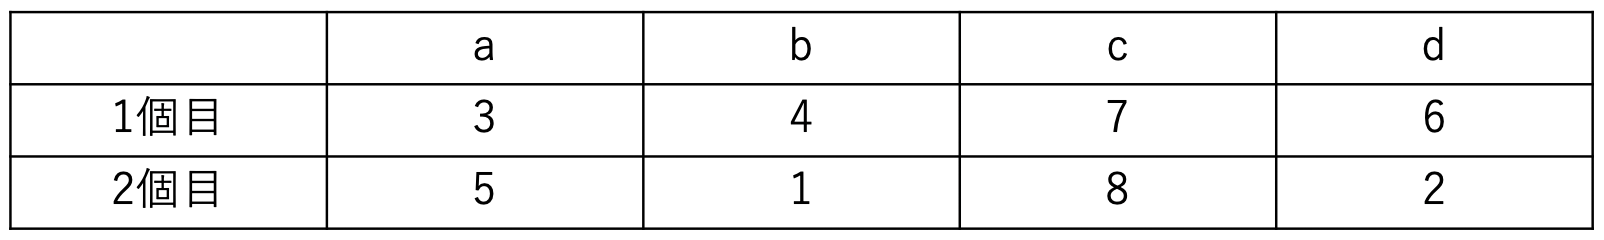
\includegraphics[width=7cm]{wariate.png}
	\caption{多重集合のハッシュ値の割り当て表}
	\label{wariate}
\end{figure}

\subsection{ハッシュ値の算出}
多重集合に対するハッシュ値算出アルゴリズムは以下のとおりである。
\begin{itemize}
	\item[1] 各要素に割り当て表の数値を割り当てる
	\item[2] 最小値をハッシュ値とする
\end{itemize}

\section{Minlistを使用した高速化}
Minlistは最小値となる候補を持っているデータ構造である。新しくデータがスライディングウインドウに入ってきたとき以下の方法でMinlistを行進する。Minlistの更新アルゴリズムを図(\ref{minlist})に示す

\begin{itemize}
	\item[1] ヒストグラムを参照して多重度を参照して割り当てる
	\item[2] 到着時刻ヒストリを参照して到着時刻によってMinlistを更新する
\end{itemize}

\begin{figure}[t]
	\centering
	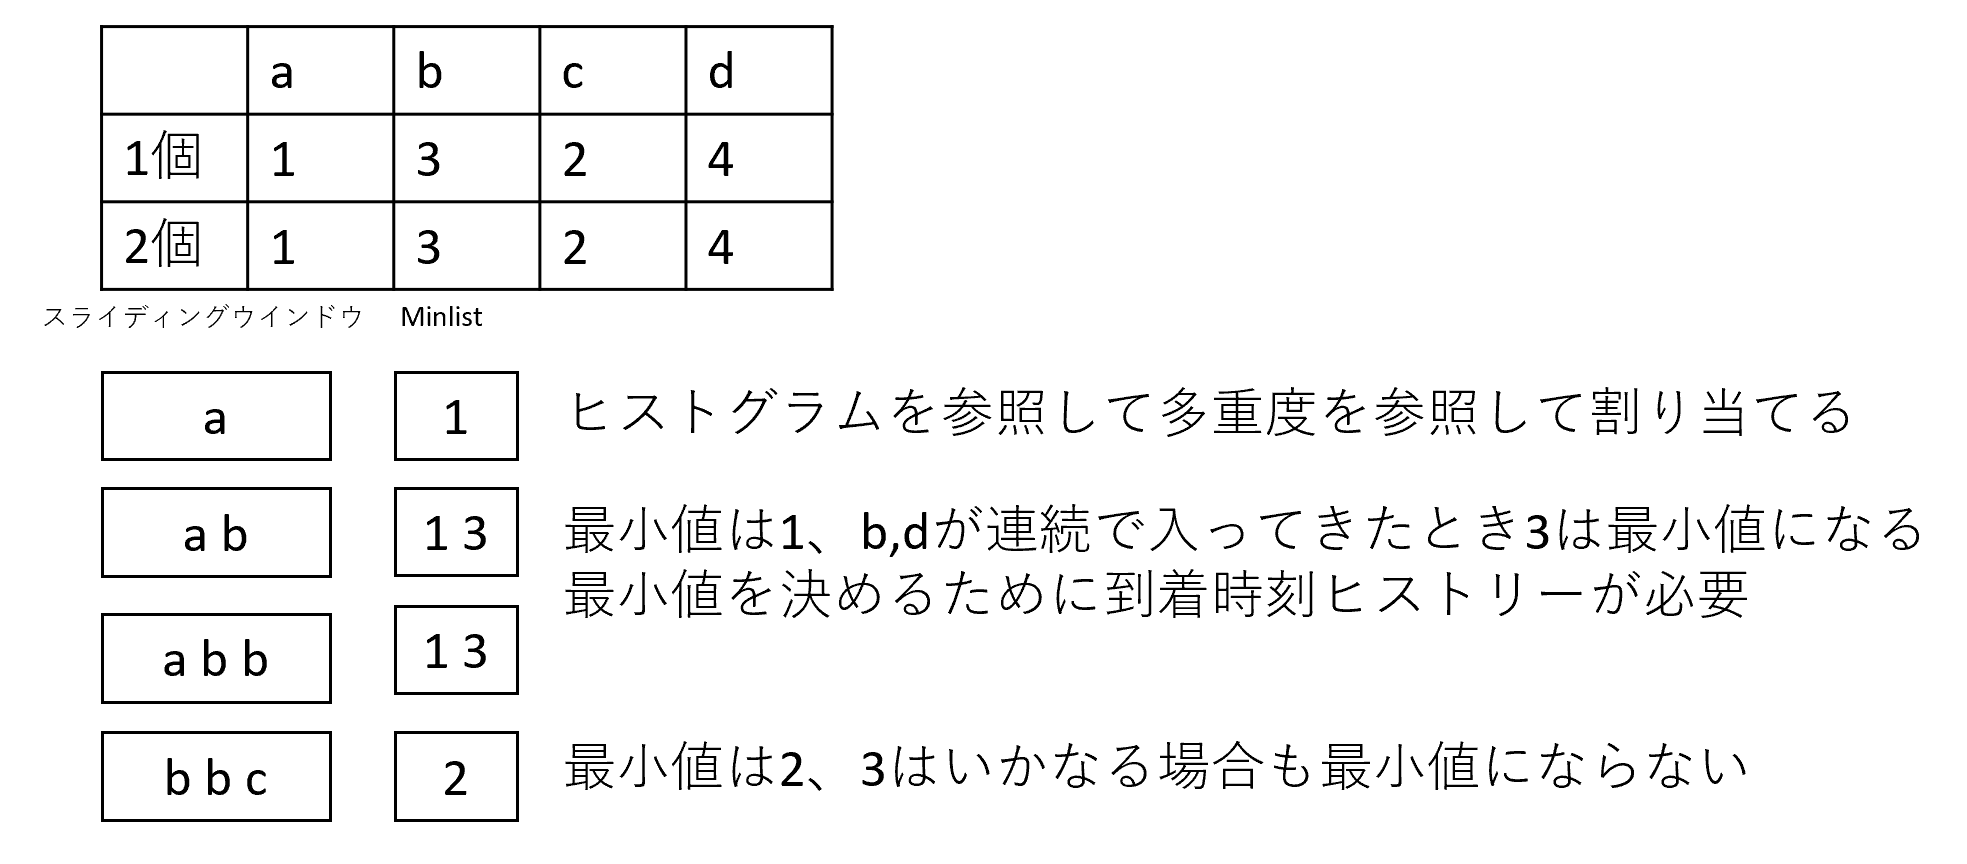
\includegraphics[width=7cm]{minlist.png}
	\caption{Minlistの更新アルゴリズム}
	\label{minlist}
\end{figure}

\subsection{要素のヒストグラム}
スライディングウインドウ内に要素の数をカウントする。多重集合である場合、同一要素が含まれているかわからないとMin-hash のハッシュ値を計算できない。

\subsection{到着時刻のヒストリ}
Minlistを作成するために必要があるため、要素がいつの時刻で到着したかリストとして所持する。リストは到着時刻が昇順で保持される。新たにウィンドウに到着した要素の到着時刻がエンキューされ、ウインドウから出ていく要素の到着時刻がデキューされる

\section{従来研究の課題}
SWMH(Sliding-Window min-Hash)は、データを保持するために空間計算量が大きい。そのため「要素のヒストグラム」「Min-Hashの割り当て表」「到着時刻のヒストリ」のデータ構造をそれぞれ小さくする。「要素のヒストグラム」は、リストのサイズが要素の種類数になる。「Min-Hashの割り当て表」は要素の種類数×多重度の上限値のサイズを持つ。「到着時刻のヒストリ」は、スライドウインドウ内の全要素の到着時刻を記録している。

\section{改善案}
「要素のヒストグラム」「Min-Hashの割り当て表」「到着時刻のヒストリ」のそれぞれに改善する方針を決めた。

\begin{itemize}
	\item[1] 要素のヒストグラム: Count-Min Sketchによる近似ヒストグラムを使う\cite{ck1}
	\item[2] Min-Hashの割り当て表: Active Indexを使って無駄な多重度を削減
	\item[3] 到着時刻ヒストリ: リストを固定長にして、使用確立が低いものはあらかじめ持たない
\end{itemize}

\subsection{Active Index}

Active Indexを用いて割り当て表に数値を割り当てるとき、多重度によって割り当て値が切り替わる境界値のインデックスと割り当て値を持つ。例は、多重度1のときに割り当て値が10、多重度2以降の割り当て値が9の場合は、1,10,2,9のように割り当て表を持つ。

\section{今後の予定}

ヒストグラムと割り当て表の削減を行う。現在は、Active IndexとCount-Min SketchをSWMHモデルに適用できるかどうか、検討している段階である。参考文献を探して、SWMHの空間計算量を削減することを目標としている。まずはSWMHの中に組み込めるか否かを疑似コードを作成して検証する。到着時刻ヒストリについてはすでに実装が完了している。

% 参考文献
\begin{thebibliography}{99}
	\scriptsize  % 参考文献以降の文字の大きさ
%\small
%	
\bibitem{RP}
三原寛寿,古賀久志, ``データストリームを対象とした動的多重集合に対する
Min-hash の高速計算アルゴリズム,`` 電気通信大学情報理工学研究, 2022
\bibitem{ck1}
Florian Hartmann, ``Count-Min Sketch,``  Google Research, 2019

\end{thebibliography}
\end{document}